%% LaTeX2e class for student theses
%% thesis.tex
%%
%% Karlsruhe University of Applied Sciences
%% Faculty of  Computer Science and Business Information Systems
%%
%%
%% Version 0.2, 2017-11-15
%%
%% --------------------------------------------------------
%% | Derived from sdqthesis by Erik Burger burger@kit.edu |
%% --------------------------------------------------------

%% Available languages: english,ngerman
%% Available modes: draft,final (see README)
\documentclass[english,final]{thesis}

% Use space between paragraphs
%\KOMAoption{parskip}{half+}

%% ---------------------------------
%% | Information about the thesis  |
%% ---------------------------------

%% Name of the author
\author{Julian Bücher}

%% Title (and possibly subtitle) of the thesis
\title{Reservation process for charging infrastructure management in the context of e-mobility}

%% Type of the thesis
\thesistype{Master Thesis}

%% Change the institute or subject area here, ``VSYS'' is default
% \myinstitute{Institute for \dots}

%% You can put a logo in the ``logos'' directory and include it here
% \grouplogo{myfile}

\reviewerone{Prof. Dr.-Ing. Zoltán Nochta}
%% reviewer two (can be omitted)
\reviewertwo{Prof. Dr. rer. nat. Heiko Körner}

%% The advisor is usually extern (can be omitted)
% \advisorone{Dipl.-Inform. C}
% The second advisor (can be omitted)
% \advisortwo{Dipl.-Inform. D}


%% Please enter the start end end time of your thesis
\editingtime{17. March 2023}{16. September 2023}

\settitle

%% --------------------------------
%% | Settings for word separation |
%% --------------------------------

%% Describe separation hints here.
%% For more details, see
%% http://en.wikibooks.org/wiki/LaTeX/Text_Formatting#Hyphenation
\hyphenation{
% me-ta-mo-del
}

%% --------------------------------
%% | Bibliography                 |
%% --------------------------------

%% Use biber instead of BibTeX, see README
\usepackage[citestyle=numeric,style=numeric,backend=biber]{biblatex}
\addbibresource{thesis.bib}

%% --------------------------------
%% | Listings                     |
%% --------------------------------

%% Basic config
\lstset{
  frame=tb,
  aboveskip=3mm,
  belowskip=3mm,
  showstringspaces=false,
  columns=flexible,
  basicstyle={\footnotesize\ttfamily},
  numbers=left,
  numberstyle=\tiny\color{gray},
  keywordstyle=\color{blue},
  commentstyle=\color{dkgreen},
  stringstyle=\color{mauve},
  breaklines=true,
  breakatwhitespace=true,
  tabsize=3,
  showlines=true
}

%% --------------------------------
%% | Glossaries                   |
%% --------------------------------

%% Use glossaries (optional)
\makeglossaries
%% Load glossary definitions from file
\loadglsentries{glossentries.tex}

%% ====================================
%% ====================================
%% ||                                ||
%% || Beginning of the main document ||
%% ||                                ||
%% ====================================
%% ====================================
\begin{document}

%% Set PDF metadata
\setpdf

%% Set the title
\maketitle

%% The Preamble begins here
\frontmatter

%% LaTeX2e class for student theses: Declaration of independent work
%% sections/declaration.tex
%%
%% Karlsruhe University of Applied Sciences
%% Faculty of  Computer Science and Business Information Systems
%%
%% --------------------------------------------------------
%% | Derived from sdqthesis by Erik Burger burger@kit.edu |
%% --------------------------------------------------------


\thispagestyle{empty}
\null\vfill
\noindent\hbox to \textwidth{\hrulefill}
\iflanguage{english}{I declare that I have developed and written the enclosed
thesis completely by myself, and have not used sources or means without
declaration in the text.}%
{Ich versichere wahrheitsgemäß, die Arbeit
selbstständig angefertigt, alle benutzten Hilfsmittel vollständig und genau
angegeben und alles kenntlich gemacht zu haben, was aus Arbeiten anderer
unverändert oder mit Änderungen entnommen wurde.}


%% ---------------------------------------------
%% | Replace PLACE and DATE with actual values |
%% ---------------------------------------------
\textbf{Karlsruhe, 16.09.2023}
\vspace{1.5cm}

\dotfill\hspace*{8.0cm}\\
\hspace*{2cm}(\theauthor)
\cleardoublepage


\setcounter{page}{1}
\pagenumbering{roman}

%% ----------------
%% |   Abstract   |
%% ----------------

%% For theses written in English, an abstract both in English
%% and German is mandatory.
%%
%% For theses written in German, a German abstract is sufficient.
%%
%% The text is included from the following files:
%% - sections/abstract

\includeabstract

%% ------------------------
%% |   Table of Contents  |
%% ------------------------
\tableofcontents

\listoffigures
\listoftables

%% ------------------------
%% | Glossary/Acronyms    |
%% ------------------------

% print glossary (optional)
\printglossary
% print acronyms (optional)
\printglossary[type=\acronymtype]

%% -----------------
%% |   Main part   |
%% -----------------

\mainmatter
% Introduction
%% LaTeX2e class for student theses
%% sections/introduction/content.tex
%%
%% Karlsruhe University of Applied Sciences
%% Faculty of  Computer Science and Business Information Systems
%%
%% --------------------------------------------------------
%% | Derived from sdqthesis by Erik Burger burger@kit.edu |
%% --------------------------------------------------------

\chapter{Introduction}
\label{ch:Introduction}

% E-Mobility and Reservations...

\section{Target}
\label{ch:Introduction:sec:Target}

The fact that subsidies and other inducements provided by the manufacturers and the state itself lead to an further increasing amount of electric vehicles \cite{afshar_literature_2020} on the streets, the extension and management of the existing charging infrastructure will become an essential part of the overall satisfaction of the \acrfull{evu} community.
Especially management or administration processes ensuring a fair and well-regulated use of the single charging possibilities is a necessary feature most implementations are missing nowadays. 
The prime example addressing this problem, is the feature gap describing a reservation of a charging point in a specified time in the future. 

Therefore reservation process for electric vehicle management inside a reduced scenario, like a company car fleet, will be used as proof of concept to demonstrate the advantages in comparison to the first-come-first-serve principle. The following sections will describe the context of the required system with their given requirements and restrictions for the tasks. First of all, a definition for electric mobility will be given, which declares the given context and its parts.

\section{SAP SE}
\label{ch:Introduction:sec:SAP SE}
SAP SE, commonly referred to as SAP, is a multinational software corporation based in Walldorf, Germany. It is one of the world's leading enterprise software companies and is renowned for its innovative solutions that help businesses manage their operations effectively. It was founded in 1972 by Dietmar Hopp, Hasso Plattner, Claus Wellenreuther, Hans-Werner Hector, and Klaus Tschira. The company's primary goal was to develop standard application software for real-time business data processing and improve the way businesses managed their operations. Beside SAP S/4HANA and SAP ERP (Enterprise Resource PLanning), SAP offers a wirde range of enterprise software products and service and catering to various business needs and industries.
With its vast global presence of offices in more than 180 countries, SAP provides solutions to customer organizations of all sizes. From small and medium-sized enterprises to multinational corporations. Beside manufacturing industries the finance and healthcare sector, as well as, retail, utilities, and public sector organizations are covered by SAP products. SAP's commitment to innovation has led to continuous improvements and advancements in its software offerings. It has embraced emerging technologies such as artificial intelligence, machine learning, Internet of Things (IoT), and blockchain to enhance its products' capabilities and address the evolving needs of businesses.

% TODO: Add additional context for e-mobility solutions



% Main part
\chapter{Fundamentals}

\section{Electric Mobility}
\label{ch:Introduction:sec:Electric Mobility}

E-mobility, short for "electromobility," refers to the use of \acrfull{ev} and other electric-powered transportation options as an alternative to conventional vehicles that run on \acrfull{ice}. As key component of the global effort to tackle climate change and achieve sustainable transportation solutions, it targets the reduction of greenhouse gas emissions, decrease dependence on fossil fuels, and mitigate the environmental impact of transportation \cite{kathiresh_e-mobility_2022}.

\subsection{Electric Vehicles}
\label{ch:Introduction:sec:Electric Mobility:Electric Vehicles}
As a fundamental cornerstone of e-mobility, \acrfullpl{ev} describe automobiles, which are powered by one or more electric engines drawing draw energy from onboard batteries or similar energy sources. \acrshortpl{ev} come in various forms, including \acrfullpl{bev}, \acrfullpl{phev}, and \acrfullpl{hev}. \acrshortpl{bev} run solely on electric power, while \acrshortpl{phev} combine an electric motor with an internal combustion engine, and \acrshortpl{hev} use both power sources but cannot be plugged in for charging \cite{kathiresh_e-mobility_2022}.

\subsection{Charging Infrastructure}
\label{ch:Introduction:sec:Electric Mobility:ssec:Charging Infrastructure}

Beside \acrshortpl{ev} the necessary charging infrastructure is one of the critical components of e-mobility. To support the widespread adoption of \acrfullpl{ev}, a robust network of \acrfullpl{cs} is essential. These stations can vary from residential charging points to public \acrfullpl{cs} installed in parking lots, streets, and commercial areas. Different charging levels exist, ranging from slow Level 1 chargers (typically used at home) to rapid \acrshort{dc} fast chargers found in public locations for quick charging \cite{afshar_literature_2020}.

On a more general level, \acrfullpl{cs} could be differentiated into the following classes:

\begin{figure}[!ht]
    \centering
    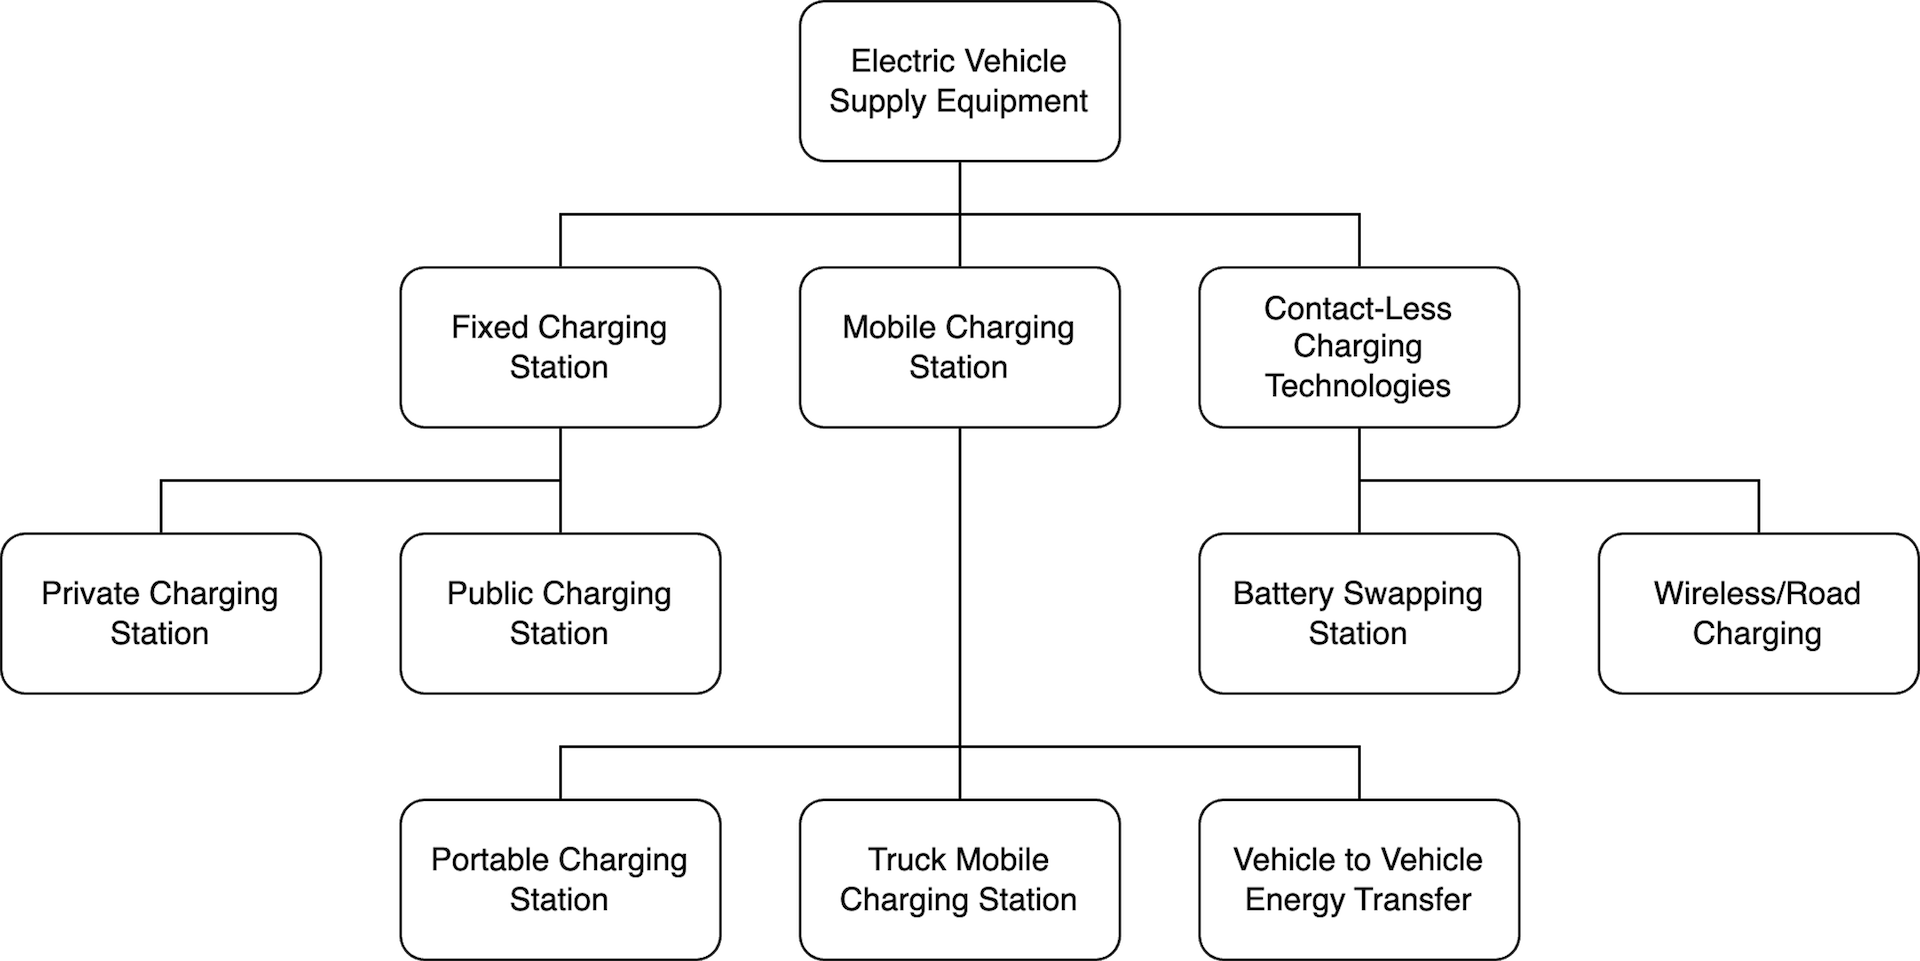
\includegraphics[scale=0.4]{resources/images/main/1_fundamentals/ChargingStationClassification.png}
    \caption{Approach of a classification of charging stations based on \cite{afshar_literature_2020}}
    \label{fig:enter-label}
\end{figure}

A more fine-granular definition is \acrfull{evse}, which refers to the infrastructure and hardware used for charging. It encompasses all the components and systems necessary to supply electric power from an electrical grid to the battery of an \acrfull{ev}, allowing it to charge and store energy for driving. Typically, it consists of the following components:

\begin{enumerate}
    \item \textbf{\acrfull{cs}}\\The physical structure or unit where the \acrshort{ev} is connected to receive electricity. \acrfullpl{cs} can vary in size and complexity, ranging from small wall-mounted units designed for home use to more extensive public \acrfullpl{cs} found in parking lots, shopping centers, and along roads.
    \item \textbf{Connector or Charging Cable}\\The cable that connects the \acrshort{ev} to the \acrfull{cs}. It contains plugs on both ends, one connecting to the vehicle's charging port and the other to the \acrfull{cs}'s outlet.
    \item \textbf{\acrfull{pms}}\\An integral part of the \acrshort{evse} that regulates the flow of electricity from the grid to the vehicle's battery. It ensures safe and efficient charging, managing the power level based on the vehicle's battery capacity and the grid's capacity.
    \item \textbf{Communication and Control System}\\This system enables communication between the \acrshort{ev}, the \acrfull{cs}, and the grid. It allows data exchange regarding charging status, electricity prices, user authentication, and other relevant information.
    \item \textbf{Payment and Authentication System}\\For public \acrfull{cs}, a payment and authentication system may be integrated into the \acrshort{evse}. This system verifies the user's identity, authorizes the charging session, and processes payment for the electricity consumed.
    \item \textbf{Safety Features}\\ \acrshort{evse} is equipped with safety features to protect users, the vehicle, and the surrounding environment. This includes features like ground fault protection, overcurrent protection, temperature monitoring, and emergency shut-off capabilities \cite{littlefuse_designing_2020}.
\end{enumerate}

Furthermore, a differentiation into specialised types of \acrshort{evse}, categorized based on the charging power and speed they offer, is possible \cite{spendiff-smith_different_2022}.

\begin{enumerate}
    \item \textbf{Level 1 Charging}\\The most basic form of \acrshort{evse}, Level 1 charging uses a standard household 120-volt AC outlet to charge the vehicle. It is typically the slowest charging option and is suitable for overnight charging at home.
    \item \textbf{Level 2 Charging}\\Level 2 charging utilizes a 240-volt AC power source, commonly found in residential and commercial settings. It provides faster charging compared to Level 1 and is commonly used for home charging setups and public charging stations.
    \item \textbf{\acrshort{dc} Fast Charging (Level 3 Charging)}\\\acrshort{dc} fast charging is the fastest charging option and operates at a higher voltage, directly charging the vehicle's battery with \acrshort{dc} power. It is commonly used in public fast-charging stations and can provide a significant amount of charge in a short time.
\end{enumerate}

\subsection{Battery Technology}
\label{ch:Introduction:sec:Electric Mobility:ssec:Battery Technology}

To store the energy required for powering electric vehicles, batteries are inevitable in the further development and acceptance of the \acrfullpl{evu} in case of range axiety and countering insufficient public charging infrastructure \cite{basmadjian_interoperable_2019}. Advancements in this technology regarding the increase in range of \acrshortpl{ev} and the reduction of charging times in combination with cost-effectiveness . Lithium-ion batteries are the most common type used in electric vehicles today, but research is ongoing to develop new battery chemistries with improved performance and longevity.

\subsection{Communication protocols}
\label{ch:Introduction:sec:Electric Mobility:ssec:Communication protocols}

To provide a general interface for information exchange between the \acrfull{cs} and the \acrfull{ev} and their users the \acrfull{oca} developed the so called \acrfull{ocpp} as standard communication protocol. It supports a standard set of functions, which could be used by the \acrfull{csms} to manage \acrshort{csms}.

\subsubsection{Open Charge Point Protocol}
\label{ch:Introduction:sec:Electric Mobility:ssec:Communication protocols:sssec:Open Charge Point Protocol}

The \acrfull{ocpp} is an industry-standard communication protocol used in \acrshort{ev} charging infrastructure to enable communication between \acrshort{evse} and \acrshort{csms}. \acrshort{ocpp} is designed to provide interoperability and seamless integration between different charging station vendors and network operators, ensuring that EV drivers can charge their vehicles at any compatible charging station. Therefore, it is an open protocol and not not proprietary to any specific manufacturer or organization. It is maintained by the \acrfull{oca}, a consortium of \acrshort{ev} charging infrastructure stakeholders, ensuring that it remains a collaborative and evolving standard \cite{noauthor_ocpp_nodate-1}.

\acrshort{ocpp} could be described as a client/server architecture. The \acrshort{evse} in this model acts as the client, while the \acrshort{csms} serves as the server. The server responds to the client's requests and manages the charging processes accordingly. This request-response model, where the client sends requests to the server, and the server responds with the appropriate information or action enables real-time communication between the \acrfull{cs} and the connected \acrfull{cms}.

As an interface for communication, two different types of protocols are used. On the one side, the WebSocket protocol for bidirectional communication, providing a persistent connection between the \acrshort{evse} and the \acrshort{cms} and allowing a faster and more efficient communication. \acrfull{soap} on the other side, is used for one-way communication.

To differentiate between particular feature sets, the \acrshort{ocpp} is versioned. The versions are illustrated as floating point numbers, which are increasing based on major or minor releases. The most recent protocol versions are \acrshort{ocpp} 1.5, \acrshort{ocpp} 1.6, \acrshort{ocpp} 2.0 and often include enhancements, additional features and bug fixes based on the increased part of the versioning.

Afterwards a collection of relevant \acrshort{ocpp} operations based on \cite{noauthor_ocpp_nodate-1}:

\begin{enumerate}
    \item \textbf{Boot Notification}\\The charging station sends a boot notification to the \acrshort{cms} when it starts up or connects to the network. This notification allows the \acrshort{cms} to identify and track the status of the charging station.
    \item \textbf{Authorize}\\Before starting a charging session, the \acrshort{evu} RFID card or other identification is sent to the central system for authorization. The \acrshort{cms} checks the driver's credentials and responds with an authorization status.
    \item \textbf{Start Transaction}\\After successful authorization, the \acrshort{cms} sends a start transaction request to initiate the charging process. The \acrshort{cs} acknowledges the request, and the charging session begins.
    \item \textbf{Meter Values}\\During the charging session, the \acrshort{cs} periodically sends meter values to the \acrshort{cms}, providing real-time information on charging status, power consumption, and other relevant data.
    \item \textbf{Stop Transaction}\\When the charging session is complete or terminated, the charging station sends a stop transaction request to the \acrshort{cms}, indicating the end of the charging process. Based on the gathered meter values, the \acrshort{cms} responds with transaction-related information, such as the total energy consumed and the charging cost.
    \item \textbf{Status Notification}\\The \acrshort{cs} may send status notifications to the \acrshort{cms} to update the current state of the charging station, such as "Available," "Charging", "Reserved", or "Faulted".
    \item \textbf{ReserveNow}\\In case a user needs an available connector on a \acrshort{cs}, he could send a "ReserveNow" request via the \acrshort{cms} to the \acrshort{cs}, which reserves one specific or at least on connector on the station for a specified duration. This connector changes from status "Available" to "Reserved" and only the user assigned to the deposited RFID card is able to charge at the connector or \acrshort{cs}.
    \item \textbf{Cancel Reservation}\\For cancelling the created reservation the user could manually send a request with the assigned reservation id to the \acrshort{cms} to free the connector again. Otherwise, the \acrshort{cs} will notify the \acrshort{cms}, if the reservation is expired.   
\end{enumerate}

\subsubsection{Open Charge Point Interface}
\label{ch:Introduction:sec:Electric Mobility:ssec:Communication protocol:sssec:Open Charge Point Interface}
\acrfull{ocpi} is an open standard protocol designed for communication between \acrshort{cs} and \acrshort{csms} or \acrshort{cpo}. It facilitates interoperability and seamless communication among various charging network operators, enabling \acrshort{ev} drivers to access charging infrastructure from different providers using a unified and standardized approach. 

Key Components of \acrshort{ocpi} are the defined endpoints, used for communication between \acrshort{cs} and \acrshortpl{cms}. These endpoints include for example functionalities like location discovery, charge point data, authorization, charging sessions, and error handling. For integrating \acrshort{ocpi} into existing software systems it is heavily based on the paradigm of \acrfull{rest}. This allows communication via standard HTTP methods utilizing \acrfull{json} as data format for transmitting information. 

The listing below provides a short overview of available features and functionalities provided by \acrshort{ocpi} \cite{noauthor_ocpiocpi_2023}:

\begin{enumerate}
    \item \textbf{Location Discovery}\\Charging networks can exchange information about available charging locations, providing details such as location coordinates, charging station types, and status.
    \item \textbf{Charge Point Data}\\Charging station data, including information on charging station availability, status, and pricing, can be accessed through OCPI.
    \item \textbf{Charging Sessions}\\OCPI supports real-time information about ongoing charging sessions, including start time, energy consumed, and current charging status.
    \item \textbf{Authorization and Authentication}\\OCPI allows EV drivers to be authenticated and authorized to access charging services through their respective CPO accounts or other authentication methods.
    \item \textbf{Remote Start/Stop Charging Sessions}\\OCPI enables the remote start and stop of charging sessions, allowing EV drivers to initiate charging sessions via their mobile apps or other remote means.
    \item \textbf{Tariff Information}\\Charging networks can share pricing and tariff information, providing transparency to EV drivers about the cost of charging at different locations.
\end{enumerate}

\subsection{Smart Charging}
\label{ch:Introduction:sec:Electric Mobility:ssec:Smart Charging}

The technology of smart charging or intelligent charging, is a systematic approach, which optimizes the charging process to be more efficient, cost-effective, and environmentally friendly. The concept of smart charging revolves around utilizing information and communication technologies to monitor and regulate the charging of electric vehicles, taking into account factors such as electricity demand, grid capacity, renewable energy availability, and preferences of single users.

One of the primary goals of this methodology is to balance the demand on the underlying grid. Charging large numbers of electric vehicles simultaneously, especially during peak hours could result in increased electricity costs or potential blackouts. Therefore, smart charging takes the current load of the grid into account and adjust the possible charging rates based on the given constraints. Prevention of overloading the grid and optimizing the use of available energy are only two side effects resulting out of this approach. 

Furthermore, the integration of \acrfull{tou} electricity plans offer different electricity rates at different times of the day. During peak hours the rates increase and gets lower during off-peak hours. This could be used to initiate scheduled charging when electricity prices are lower, saving the money for the \acrshortpl{evu} and reducing the strain on the grid. 

This effect could be doubled by leveraging real-time data on renewable energy availability, such as solar and wind power. Smart Charging systems could prioritize charging when enough electricity out of renewables is available. This not only reduces greenhouse gas emissions associated with charging \acrshortpl{ev} but also maximizes the utilization of clean and sustainable energy sources.

Beside the unidirectional charging method originally called \acrfull{v1g}, the approach of \acrfull{v2g} enables smart charging systems to charge bidirectionally between the \acrshortpl{ev} battery and the grid. During times of high demand, \acrshortpl{ev} with sufficient battery capacity can supply energy to the grid. This concept turns \acrshortpl{ev} into mobile energy storage units, enhancing grid stability and resiliency.

To offer all these functions, smart charging relies heavily on data connectivity and communication between the single \acrshortpl{cs}, the \acrshortpl{ev} and the underlying grid, which makes it vulnerable for malign third-party entities as well. On the other side, these aspects are capable of contributing to an overall improved grid management. Grid operators could gain insights into electricity demand patterns and plan grid upgrades accordingly.

\section{Reservation Systems}
\label{ch:Introduction:sec:Reservation Systems}

As per particulars described below, a reservation system could be described by definition as a software application or platform that facilitates the process of booking and securing limited services, resources, or accommodations in advance. It is commonly used in various industries, including travel, hospitality, transportation, entertainment, and more, to manage and streamline the reservation process for customers or clients. It allows the reduction of administrative workload and enhance the users experience in case of streamlined processes. 

Key features and functionalities of a reservation system typically include:

\begin{enumerate}
    \item \textbf{Booking and Scheduling}\\Users can view available dates, times, or slots and make reservations for specific services, activities, or resources. The system ensures that conflicting bookings do not occur.
    \item \textbf{Real-Time Availability}\\The reservation system shows real-time availability, meaning users can see immediately if the desired service or resource is available for the chosen date and time.
    \item \textbf{User Registration and Authentication}\\Users may need to create an account or log in to make reservations. This feature helps in personalizing the experience, storing reservation history, and providing loyalty rewards.
    \item \textbf{Online Payments}\\Reservation systems often include secure payment processing to enable users to pay for their bookings online using credit/debit cards, digital wallets, or other payment methods.
    \item \textbf{Confirmation and Notifications}\\After making a reservation, users receive a confirmation email or notification, which serves as proof of the booking and may include relevant details like booking ID, date, time, and location.
    \item \textbf{Cancellation and Modification}\\Users can cancel or modify their reservations within a specified timeframe. The system may have cancellation policies and penalties for late cancellations.
    \item \textbf{Inventory Management}\\For industries like hotels or rental services, the reservation system helps manage inventory and ensures that resources or rooms are not overbooked.
    \item \textbf{Reporting and Analytics}\\The system may generate reports on booking trends, revenue, occupancy rates, and other performance metrics for businesses to analyze and optimize operations.
    \item \textbf{Integration with Other Systems}\\A reservation system may integrate with other software or systems, such as customer relationship management (CRM) software, payment gateways, or channel managers.
\end{enumerate}

\subsection{Reservation}
\label{ch:Introduction:sec:Reservation Systems:ssec:Reservation}


%% LaTeX2e class for student theses
%% sections/2_chapter/req_eng_and_pr_design.tex
%%
%% Karlsruhe University of Applied Sciences
%% Faculty of  Computer Science and Business Information Systems
%%
%% --------------------------------------------------------
%% | Derived from sdqthesis by Erik Burger burger@kit.edu |
%% --------------------------------------------------------

\chapter{Requirements Engineering}
\label{ch:Requirements Engineering}

Based on the existing concepts and design proposals elaborated in the previous chapter, this work has the target to design and implement a reservation process considering a problem statement described in detail as part of the following section. 
After an analysis of the identified actors and use cases of the outlined scenario, requirements for the process design will be derived and formalized in diagrams with the Business Process Modelling Notation \cite{noauthor_bpmn_nodate} and Unified Modelling Language 2.0 \cite{noauthor_welcome_nodate}.
Resulting in a reservation process design describing the interactions with its users and the behavior in different situations will stay at the end of this chapter. 

\section{Scenario}
\label{ch:Requirements Engineering:sec:Scenario}

For the conceptional design of the process a scenario will be used, to simulate different actors and their needs with regard to the criteria of usability and accessibility. Afterwards these actors will be used as personas to formulate use cases and the interactions with the system. 
Beginning with the selection of the location, the subsequent setting takes place. Appropriate to its functionality as partner of the underlying project, which is artifact of this work, the \acrfull{hka} with focus on three of the site areas within the city of Karlsruhe is selected.
The designation and the location within the city are irrelevant for this scenario and will not be further described.
Each site represents a separate campus with the corresponding students, their lecturers and staff of the \acrshort{hka}, which use different transport facilities to bridge the distance between the campuses themselves or their homes. 
Beside the people arriving via public transport, the author assumes that in case of subventions of electric vehicles in the federal republic of Germany, a growing amount of people have acquired electric vehicles for their daily transportation. 
The parking lots at the different campus sites offer a limited amount of \acrfull{cs}s to provide charging capabilities to a subset of \acrfull{evu}s arriving there. 
Regarding the management of the existing charging infrastructure, the \acrshort{hka} uses an open source solution, which consists of a user interface accessible through a browser and used by administrative departments of the different campuses, a mobile client for the end users and a backend system procuring the communication with the facilities. 
By now, the administrator or the end user does not have an opportunity to reserve a charging station connector on behalf of a specific user or for themselves.
Just the enabling and disabling of specific charging connectors or the whole charging station is implemented.
As an implication of this restriction, a "first-come-first-serve" mentality among the \acrshort{evu}s will be induced and a equitable usage of the existing charging possibilities is not given anymore.
To prohibit such a invidious situation the mentioned solution should furnish a reservation functionality allowing a fine grained distribution between public accessible \acrshort{cs} connectors and a subset, which is prohibited for public use and for \acrshort{evu}s with existing reservations only.

\section{Actors}
\label{ch:Requirements Engineering:sec:Actors}

Next, the scenario needs a set of actors, which could be used as personas for describing different use cases, the system has to provide in case of an interaction with the given actor. 
In case of a university, as described above, the author selected a subset of possible groups of people, existing in such a context. 
Therefore, four groups were selected, representing a required minimum for constructing viable cases and edge cases. Each group has a representative in form of a persona, pictured by a fictional person in combination with a role inside the system itself.
For a better understanding of the role collection provided by the system, the following table \ref{tab:system_role_collection} introduces the relevant roles, shortages and a brief description.

\begingroup
\setlength{\tabcolsep}{10pt} % Default value: 6pt
\renewcommand{\arraystretch}{1.5} % Default value: 1
\begin{table}[h!]
    \centering
    \begin{tabular}{c|c|c|m{6cm}}
        Role & System & Shortage & Description \\
        \hline
        Basic & \verb|BASIC| & \verb|B| & Standard user without administrative privileges \\
        Admin & \verb|ADMIN| & \verb|A| & User with administrative privileges inside a tenant organisation \\
        Super Admin & \verb|SUPER_ADMIN| & \verb|S| & User with extended administrative privileges for creation of tenant organizations and initialization of templates for cars and charging stations \\
        Demo & \verb|DEMO| & \verb|D| & Demo user for test purposes \\
    \end{tabular}
    \caption{Role collection provided by the system}
    \label{tab:system_role_collection}
\end{table}
\endgroup

The identified groups of the scenario will be part of the next listing. Therefore, the group will be described and in the next step assigned to a specific role in the context of the case.

\begin{description}
    \item[Student] Personas representing students studying at the \acrshort{hka}. Mainly they spent time at the main campus, where all lectures and the attendant exercises take place. To travel between their home and the university, beside using the train, they drive with electric vehicles or plug-in hybrids to minimise their carbon footprint. Due to the fact, that the amount of students with EVs outnumber the capacity of charging stations at the different sites of the \acrshort{hka}, this group does not have the possibility to reserve a charging station for recharging their vehicles. Students have to arrive early to catch one of the charging points, which are free/public available.
    \item[Staff] Set of personas belonging to the staff of \acrshort{hka}. They have different roles inside the university, which could be lecturer, service worker, cleaner or librarian for example. Unlike students, the staff has the option to request a reservation. This reservation request will be processed by the secretary of the institution or directly via the janitor. By permitting the request the staff members get a reservation for a charging point/connector at the specified site of \acrshort{hka}. In case of days of or working from home, the reservations could be canceled. Otherwise the janitor or the secretaries could do this via the CSMS admin dashboard. As a rule of thumb this kind of reservations are recurring.
    \item[Janitor] This group represents a special subset of \acrshort{hka} staff. Beside managing and maintaining parts of the physical infrastructure, they are responsible for service offerings regarding the charging stations installed on the three different campus locations. To observe the connected infrastructure, they have access to the administration dashboard provided by the open source solution and are responsible for handling incoming reservation requests. 
    \item[Secretary] In contrast to the group of janitors, the secretary is the administrative counterpart for managing the data and internal processes inside the \acrshort{hka}. Beside paperwork regarding approvals for new students, updating the annual records and processing requests from students, they are organizing events and supervise external visitors. Therefore, staff members inside the secretary needs occasionally access to the charging station management platform to guarantee charging possibilities to guests arriving at the different campus locations.
\end{description}

\begin{table}[h!]
    \centering
    \begin{tabular}{c|c}
        Group & Role \\
        \hline
        Student & \verb|BASIC| \\
        Staff & \verb|BASIC| \\
        Janitor & \verb|ADMIN| \\
        Secretary & \verb|ADMIN|
    \end{tabular}
    \caption{Role mapping of the system roles to the different groups identified in the scenario described in \ref{ch:Requirements Engineering:sec:Scenario}}
    \label{tab:role_mapping_scenario}
\end{table}


\subsection{Personas}
\label{ch:Requirements Engineering:sec:Personas}

For a better understanding of the different roles and their requirements they concern by using the system, a set of personas is described below. They will be used as identifier and a representative for the user group they are assigned to. A detailed description of the four different personas and their circumstances follows afterwards.

\subsection{Lisa Knaus}
\label{ch:Requirements Engineering:sec:Personas:ssec:Lisa Knaus}

Lisa Knaus is a student of the \acrshort{hka}. She studies Computer Science in third semester and lives in her hometown Untergrombach. Since she was 18 years old, she used a car as main transport medium. For travelling between her location to study and her hometown she uses the family car, which is an \acrfull{fev} without an \acrfull{ice}. The battery health of her car allows her to reach the main campus and return home after lectures, without a need to recharge. But occasionally she forgot to charge her car at home and need to recharge her vehicle at the \acrshort{hka}. For using the charging service at the parking lots on-site, she submitted a request for account creation at the secretary of her university. Since then, she uses the offered service from time to time, if she arrives early enough to catch a free charging station.

\subsection{Holger Starke}
\label{ch:Requirements Engineering:sec:Personas:ssec:Holger Starke}

Holger Starke is part of the maintenance team taking care of the server landscape the \acrshort{hka} hosting its internal applications and fostering their user databases. By virtue of the subvention of electric vehicles by the state and his employer he bought a \acrshort{fev} last year. Despite the fact of his short travelling distance between his apartment in Karlsruhe and his workplace, he does not have the possibility to recharge the \acrshort{ev} at home. So he has to use the available charging stations at the different campus locations the \acrshort{hka} offers. However, sometimes if he has to switch between the different campuses very often, the available \acrshort{cs} are already taken.

\subsubsection{Dieter Krause}
\label{ch:Requirements Engineering:sec:Personas:ssec:Tom Krause}

Dieter Krause works as a janitor at \acrshort{hka} for five years now. Before taking over the responsibility for the charging infrastructure management and maintenance he acted as carrier for book orders between the various university libaries in Karlsruhe. For transportation purposes he used a van owned by his employer to gather the book orders at one library and drive them to the others. Because of short traveling distances inside Karlsruhe the \acrshort{hka} provided him \acrshort{fev} for reducing carbon dioxide emissions. To fulfill his new purpose as service worker for the charging stations he could further utilize the old van. In contrast to the other \acrshort{evu}s Tom has the option to charge his van on a exclusive \acrshort{cs}, which is dislocated from the other charging infrastructure. Even at days with high emergence of student vehicles on the public parking lots, he could recharge the batteries of the van. 

\subsection{Nadine Funke}
\label{ch:Requirements Engineering:sec:Personas:ssec:Nadine Funke}

Nadine Funke is a secretary at the administration office of \acrshort{hka} for three years. Formerly she worked at the public administration office in Karlsruhe and already have experience with the complex of problems regarding the charging of \acrshort{ev}s at public charging infrastructure. Beside the maintenance staff, she got access to the charging station management dashboard for blocking \acrshort{cs}s in consideration of arriving guests. Till now, she has to select the specific charging station and the according connector for blocking and needs to enable it again, if the guest has arrived. 

\subsection{Use Cases}
\label{ch:Requirements Engineering:sec:Use Cases}

Analysing the scenario described in \ref{ch:Requirements Engineering:sec:Scenario}, the following use cases were identified. In terms of clarity and better understanding of the assignment of use case with persona group, the following use case diagrams are describing the use cases in terms of normal users with the role \verb|BASIC| in separation to the use cases administrative users with the role \verb|ADMIN| care about. Afterwards a detailed description of the single cases will follow.

\begin{figure}[h!]
    \centering
    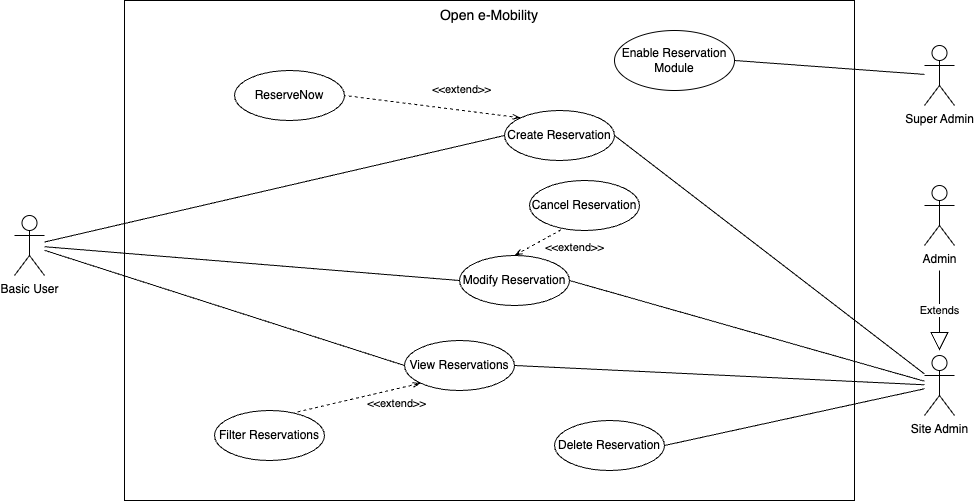
\includegraphics[scale=0.4]{resources/images/main/2_requirements/UseCases.png}
    \caption{Use Cases for users of Open e-Mobility}
    \label{fig:uc_basic_users}
\end{figure}

\begingroup
\setlength{\tabcolsep}{10pt} % Default value: 6pt
\renewcommand{\arraystretch}{1.5} % Default value: 1
\begin{table}[!ht]
    \centering
    \begin{tabular}{m{3.5cm}|c|m{3cm}|m{4cm}}
        Use Case & Shortage & Corresponding Persona & Description \\
        \hline
        Book a reservation & UC1 & Student, Staff, Janitor, Secretary & TODO: \\
        Cancel a reservation & UC2 & Student, Staff, Janitor, Secretary & TODO: \\
        Edit a reservation & UC3 & Student, Staff, Janitor, Secretary & TODO: \\
        Start a transaction & UC4 & Student, Staff, Janitor, Secretary & TODO: \\
        Stop a running transaction & UC5 & Student, Staff, Janitor, Secretary & TODO: \\
        Book a reservation on behalf of another user  & UC6 & Student, Staff, Janitor, Secretary & TODO: \\ 
        Cancel a reservation on behalf of another user & UC7 & Janitor, Secretary & TODO: \\
        Enable charging station for reservation & UC8 & Janitor, Secretary & TODO: \\
        Disable charging station for reservation & UC9 & Janitor, Secretary & TODO: \\
    \end{tabular}
    \caption{Use Case overview with assignment to the corresponding personas and a brief description}
    \label{tab:use_case_overview}
\end{table}
\endgroup

\chapter{Approach}
\label{ch:Approach}

\section{Theoretical Part}
\label{ch:Approach:sec:Theoretical Part}
TODO: Describing the approach for analyzing the literature and extracting individual research for utilizing in the practical part.
\dots

\section{Practical Part}
\label{ch:Approach:sec:Practical Part}

\dots
\chapter{Literature Review}
\label{ch:Literature Review}

\section{Related Work}
\label{ch:Literature Review:sec:Related Work}
\chapter{Process Design}
\label{ch:Process Design}

\section{Entities}
\label{ch:Process Design:sec:Entities}

% \begin{figure}
%     \centering
%     \includegraphics{}
%     \caption{Caption}
%     \label{fig:enter-label}
% \end{figure}

\section{Implemented Use Cases}
\label{ch:Process Design:sec:Implemented Use Cases}

% \begin{figure}
%     \centering
%     \includegraphics{}
%     \caption{Caption}
%     \label{fig:enter-label}
% \end{figure}

\subsection{Create Reservation}
\label{ch:Process Design:sec:Implemented Use Cases:ssec:Create Reservation}

% \begin{figure}
%     \centering
%      \begin{subfigure}[b]{0.3\textwidth}
%          \centering
%          \includegraphics[width=\textwidth]{graph1}
%          \caption{$y=x$}
%          \label{fig:enter-label}
%     \end{subfigure}
%      \hfill
%      \begin{subfigure}[b]{0.3\textwidth}
%          \centering
%          \includegraphics[width=\textwidth]{graph1}
%          \caption{$y=x$}
%          \label{fig:enter-label}
%     \end{subfigure}
%      \hfill
% \end{figure}

\subsection{Update Reservation}
\label{ch:Process Design:sec:Implemented Use Cases:ssec:Update Reservation}

% \begin{figure}
%     \centering
%      \begin{subfigure}[b]{0.3\textwidth}
%          \centering
%          \includegraphics[width=\textwidth]{graph1}
%          \caption{$y=x$}
%          \label{fig:enter-label}
%     \end{subfigure}
%      \hfill
%      \begin{subfigure}[b]{0.3\textwidth}
%          \centering
%          \includegraphics[width=\textwidth]{graph1}
%          \caption{$y=x$}
%          \label{fig:enter-label}
%     \end{subfigure}
%      \hfill
% \end{figure}

\subsection{Delete Reservation}
\label{ch:Process Design:sec:Implemented Use Cases:ssec:Delete Reservation}

% \begin{figure}
%     \centering
%      \begin{subfigure}[b]{0.3\textwidth}
%          \centering
%          \includegraphics[width=\textwidth]{graph1}
%          \caption{$y=x$}
%          \label{fig:enter-label}
%     \end{subfigure}
%      \hfill
%      \begin{subfigure}[b]{0.3\textwidth}
%          \centering
%          \includegraphics[width=\textwidth]{graph1}
%          \caption{$y=x$}
%          \label{fig:enter-label}
%     \end{subfigure}
%      \hfill
% \end{figure}

\subsection{Cancel Reservation}
\label{ch:Process Design:sec:Implemented Use Cases:ssec:Cancel Reservation}

% \begin{figure}
%     \centering
%      \begin{subfigure}[b]{0.3\textwidth}
%          \centering
%          \includegraphics[width=\textwidth]{graph1}
%          \caption{$y=x$}
%          \label{fig:enter-label}
%     \end{subfigure}
%      \hfill
%      \begin{subfigure}[b]{0.3\textwidth}
%          \centering
%          \includegraphics[width=\textwidth]{graph1}
%          \caption{$y=x$}
%          \label{fig:enter-label}
%     \end{subfigure}
%      \hfill
% \end{figure}

\subsection{Schedule Reservation}
\label{ch:Process Design:sec:Implemented Use Cases:ssec:Schedule Reservation}

% \begin{figure}
%     \centering
%     \includegraphics{}
%     \caption{Caption}
%     \label{fig:enter-label}
% \end{figure}

\subsection{Expire Reservation}
\label{ch:Process Design:sec:Implemented Use Cases:ssec:Expire Reservation}

% \begin{figure}
%     \centering
%     \includegraphics{}
%     \caption{Caption}
%     \label{fig:enter-label}
% \end{figure}

\subsection{Free reserved connectors}
\label{ch:Process Design:sec:Implemented Use Cases:ssec:Free reserved connectors}

% \begin{figure}
%     \centering
%     \includegraphics{}
%     \caption{Caption}
%     \label{fig:enter-label}
% \end{figure}

\section{Not Implemented Use Cases}
\label{ch:Process Design:sec:Not Implemented Use Cases}

\subsection{Smart Charging Integration}
\label{ch:Process Design:sec:Not Implemented Use Cases:sec:Smart Charging}

%% LaTeX2e class for student theses
%% sections/content.tex
%%
%% Karlsruhe University of Applied Sciences
%% Faculty of  Computer Science and Business Information Systems
%%
%% --------------------------------------------------------
%% | Derived from sdqthesis by Erik Burger burger@kit.edu |
%% --------------------------------------------------------

\chapter{Implementation}
\label{ch:Implementation}

\section{Implemented Use Cases}
\label{ch:Implementation:sec:Implemented Use Cases}

Afterwards, the implemented use cases will be described in details.

\subsection{Create Reservation}
\label{ch:Implementation:sec:Implemented Use Cases:ssec:Create Reservation}

\begin{figure}[!ht]
    \centering
    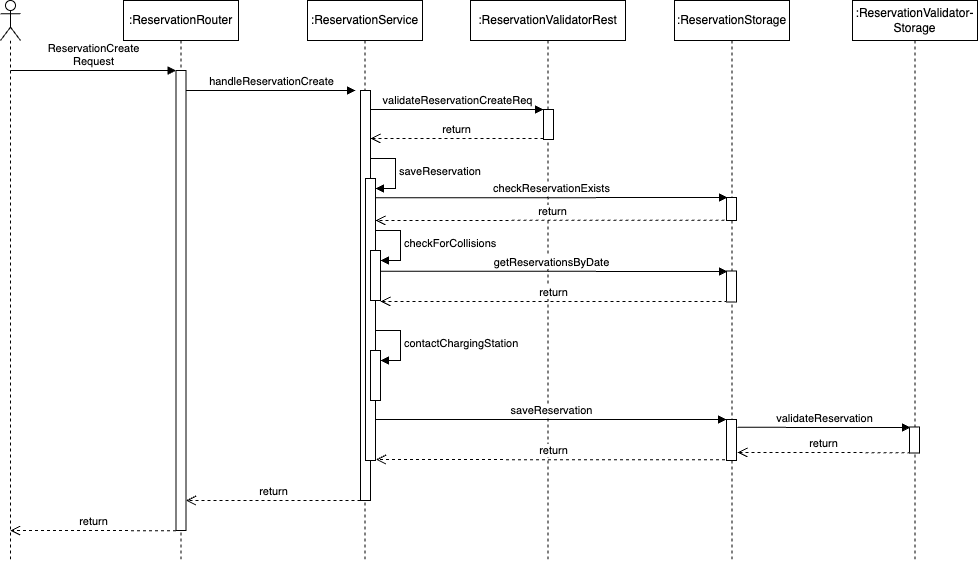
\includegraphics[scale=0.4]{resources/images/main/6_implementation/ReservationCreate.png}
    \caption{Flow of information through the single components of the backend service}
    \label{fig:create-reservation-seq-flow}
\end{figure}

\subsection{Update Reservation}
\label{ch:Implementation:sec:Implemented Use Cases:ssec:Update Reservation}


\begin{figure}[!ht]
    \centering
    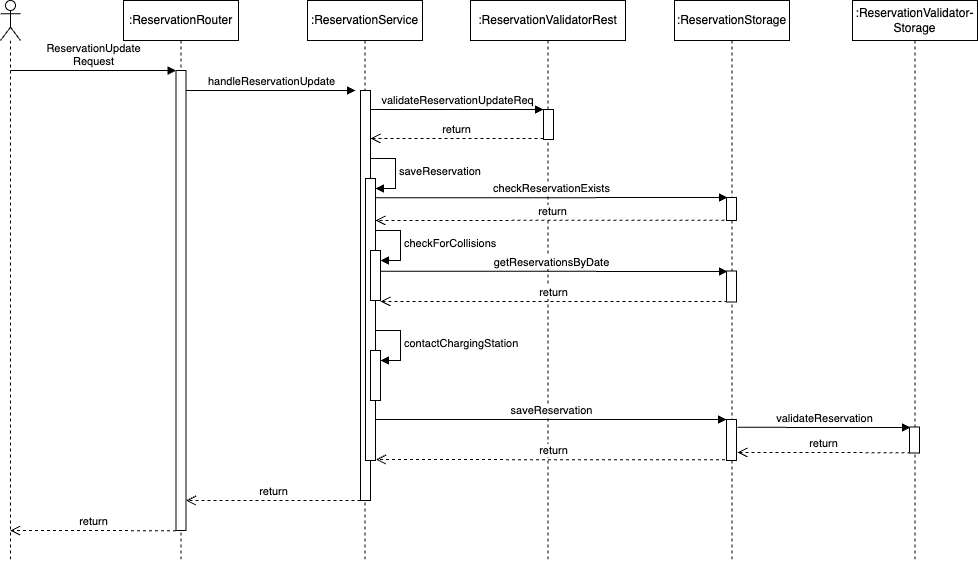
\includegraphics[scale=0.4]{resources/images/main/6_implementation/ReservationUpdate.png}
    \caption{Flow of information through the single components of the backend service}
    \label{fig:update-reservation-seq-flow}
\end{figure}

\subsection{Delete Reservation}
\label{ch:Implementation:sec:Implemented Use Cases:ssec:Delete Reservation}

\begin{figure}[!ht]
    \centering
    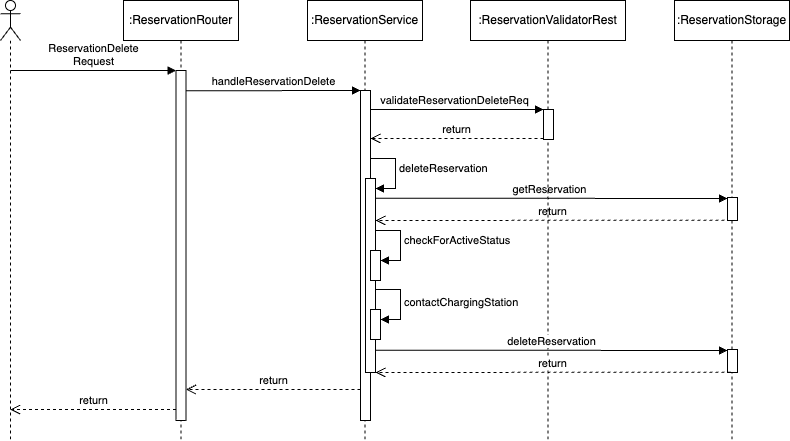
\includegraphics[scale=0.4]{resources/images/main/6_implementation/ReservationDelete.png}
    \caption{Flow of information through the single components of the backend service}
    \label{fig:delete-reservation-seq-flow}
\end{figure}

\subsection{Cancel Reservation}
\label{ch:Implementation:sec:Implemented Use Cases:ssec:Cancel Reservation}


\begin{figure}[!ht]
    \centering
    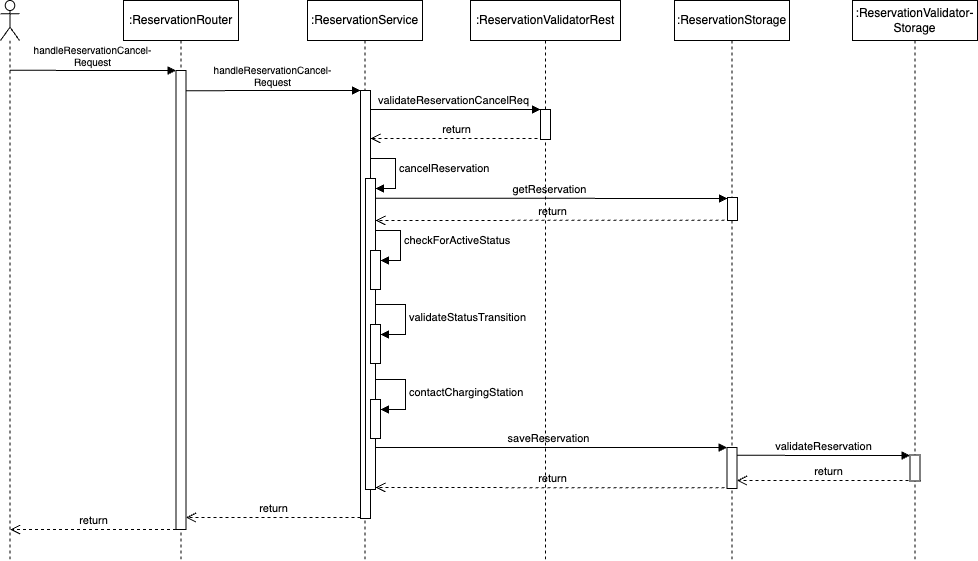
\includegraphics[scale=0.4]{resources/images/main/6_implementation/ReservationCancel.png}
    \caption{Flow of information through the single components of the backend service}
    \label{fig:cancel-reservation-seq-flow}
\end{figure}

\subsection{Schedule Reservation}
\label{ch:Implementation:sec:Implemented Use Cases:ssec:Schedule Reservation}


\begin{figure}[!ht]
    \centering
    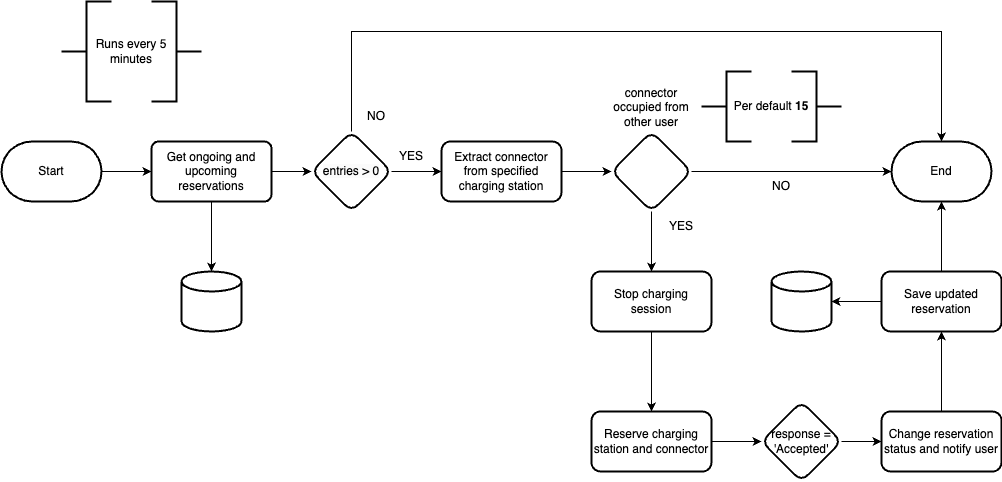
\includegraphics[scale=0.4]{resources/images/main/6_implementation/scheduler/SynchronizeReservation.png}
    \caption{Flow of information through the single components of the backend service}
    \label{fig:schedule-reservation-flow}
\end{figure}

\subsection{Expire Reservation}
\label{ch:Implementation:sec:Implemented Use Cases:ssec:Expire Reservation}

\dots

\subsection{Free reserved connectors}
\label{ch:Implementation:sec:Implemented Use Cases:ssec:Free reserved connectors}

\begin{figure}[!ht]
    \centering
    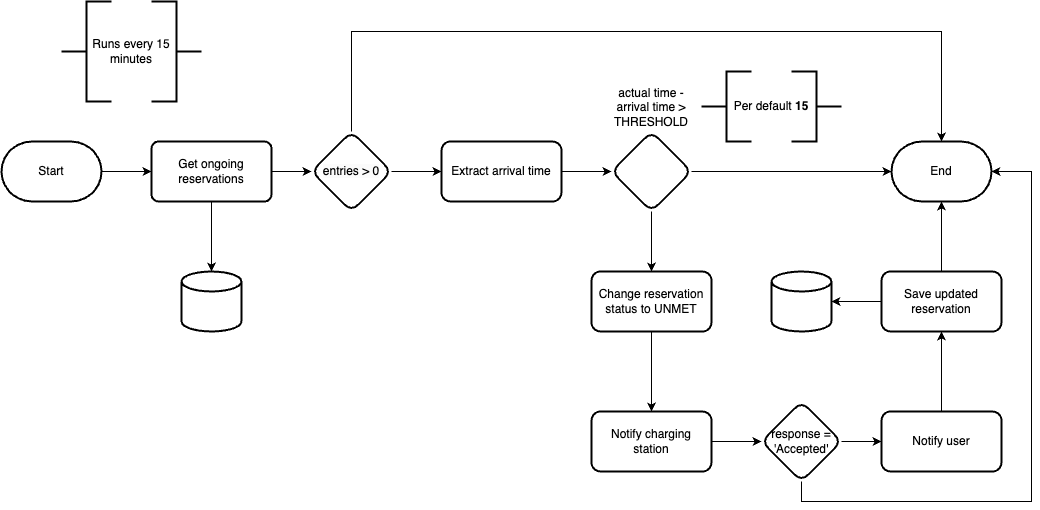
\includegraphics[scale=0.4]{resources/images/main/6_implementation/scheduler/CancelUnmetReservation.png}
    \caption{Flow of information through the single components of the backend service}
    \label{fig:free-connector-flow}
\end{figure}
%% LaTeX2e class for student theses
%% sections/content.tex
%%
%% Karlsruhe University of Applied Sciences
%% Faculty of  Computer Science and Business Information Systems
%%
%% --------------------------------------------------------
%% | Derived from sdqthesis by Erik Burger burger@kit.edu |
%% --------------------------------------------------------

\chapter{Analysis and Validation}
\label{ch:Analysis and Validation}

\dots

% Conclusion 
%% LaTeX2e class for student theses
%% sections/conclusion.tex
%%
%% Karlsruhe University of Applied Sciences
%% Faculty of Computer Science and Business Information Systems
%%
%% --------------------------------------------------------
%% | Derived from sdqthesis by Erik Burger burger@kit.edu |
%% --------------------------------------------------------


\chapter{Resume and Outlook}
\label{ch:Resume and Outlook}

Summarizing the results achieved in the development of a comprehensive reservation system for the management of charging infrastructure, this final chapter provides a resume concluding the tasks of this work. 
Also, a consideration of the contribution to the results already elaborated in the literature is given. 
Together with these retrospective views, this chapter concludes by providing an outlook on future possibilities for this category of system and proposing directions for future work. \\
%% --------------------------------------------------------
%% Resume
%% --------------------------------------------------------
\noindent Especially the administration and maintenance of charging infrastructure face several constraints that are not only determined by existing standards or technical limitations. A frequently underestimated fact is the process-related impediments to ensure the intended behaviour from the system, the charging environment and the driver.
Beyond the behaviour of the individual system components and the corresponding actors, the exchange of information between the components is another aspect that needs to be considered in the process of designing an extensible system that should allow both the interconnectivity of several stations from different manufacturers and the ease of access by users.
Therefore, the proposed design and development of a comprehensive solution aims to address all these concerns by extending one of the available communication standards to provide a \acrshort{poc} that demonstrates at least a basic set of features across multiple applications.
Concerning the fulfilment of the goals initially stated at the beginning of this work, this approach is at least capable of handling charging appointments according to the \acrshort{ocpp} standard in version 1.6 and is therefore applicable for the intention of being used within universal scenarios dealing with the problem of coordinated \acrshort{cs} allocation. 
Besides the standard reservation method, which only permits immediate blocking of a connector, extending the functionality of \acrshort{ocpp} not only allows users to make arrangements in advance for future charging sessions but also recurring bookings not accommodated by other system approaches during the time of this research.
Mitigating the inconvenience of making a booking for every single day, is a more convenient method for drivers seeking to use a particular station over a longer period of time, spanning multiple days. This also addresses the needs of the actors, certainly in the conceptualised scenario of this work, where the actors have dedicated parking spaces that they belong to.
More generally, these features are also applicable to car parks owned by providers who, in the mind of the author, need to explicitly control the individual parking spaces equipped with \acrshortpl{cs}.
Supported by the introduction of additional states describing the reservation life cycle, both the administrator and user gain more precise control over the created entity. At the same time, this provides a much more detailed way of monitoring and management.  \\
%% --------------------------------------------------------
%% Scientific Contribution
%% --------------------------------------------------------
\noindent Taking into account the aspects listed above, the previously reviewed proposal for a systematic approach regarding \acrshortpl{cs} allocation allows the following contributions in terms of supporting the existing references.
By introducing requirements for specific background processes, such as managing non-arriving \acrshortpl{evu} and initiating mitigation processes prior to the start of a charging session at stations with pending reservations, the range of scenarios respected in other projects could be extended.
Alongside highlighting problematic situations, this documentation provides suggestions for resolving these conflicts using the options typically available to that system.
This ensures a higher degree of enforcing arriving reservations and a more automated approach to managing infrastructure availability, avoiding unnecessary blockages, due to the background processes mentioned above. 
Combined with the additional life cycle states describing the validity of a booking and detailed consideration of relevant error cases, including both the exceptions from the processes and those from the charging infrastructure, a new terminology as well as attention to scenarios requiring more complex combinations were introduced.
Furthermore, the elaborated entities describe a suitable way to encapsulate the request objects of the base standard, which also serves as a guideline for further extensions. \\
%% --------------------------------------------------------
%% Outlook
%% --------------------------------------------------------
\noindent Switching the perspective from solely focusing on managing stations or infrastructure at a specific location to considering the possibility of connecting different infrastructures, creating a network of interconnected stations communicating via a common backbone, the problem most highlighted in the context of \acrshort{emobility}, also known as 'range anxiety' \cite{rauh_understanding_2015}, could also be addressed through the use of reservation systems.
As suggested in the literature by \cite{zarkeshev_charging_2018}, enabling \acrshortpl{ev} to share data on their current battery status and charging needs directly with the station, together with the use of roaming capabilities that build a heterogeneous networked infrastructure with the ability to reserve the stations along the route, could alleviate such fears.
Moreover, linking several \acrshortpl{cso}, \acrshortpl{cpo} and \acrshortpl{emsp} would lead to a higher acceptance of their services by the \acrshortpl{evu}, and thus to an increase in both usage and profits.
This could facilitate the development of new areas, offering numerous business prospects, by supporting the installation of stations and expanding the existing infrastructure.
Nevertheless, it is important to take into account the increased load on the grid that would be caused by this. However, by knowing the amount of time that the \acrshort{ev} will eventually park at the \acrshort{cs} location, combined with the current battery state, the amount of energy required to recharge to a full state of charge could be determined.
The remaining unneeded power could therefore be used by smart charging scenarios such as \acrshort{v2g}, which aims to support overall grid stability using excessive power from \acrshortpl{ev}.
Other applications could include \acrshort{v2b} to return energy to the building where the power unit is located, \acrshort{v2h} to replace the building by the driver's home, or \acrshort{v2x} to cover various targets.
In order to further promote the adoption of \acrshortpl{ev}, enhance the corresponding infrastructure and provide support for all the scenarios mentioned, the need for future development work in this area is obvious. \\
%% --------------------------------------------------------
%% Future Work
%% --------------------------------------------------------
\noindent Regarding the purpose of subsequent elaborations, below are some examples that the author of this work considers significant and possibly useful for future research. 
First to be mentioned are the fundamental constraints imposed by the state of the grid, which require special attention. Without a functional grid to power the relevant stations and vehicles, further developments in energy storage and infrastructure observation are pointless.
Therefore, the simulations already in existence, taking into account the different types of elaborated reservations to measure their impact on the journey duration and overall comfort, introduced by Basmadjian et al. in \cite{basmadjian_reference_2020,basmadjian_interoperable_2019}, could be used as groundwork to create scenarios specifically to simulate the effects of reservations to cushion peek loads using \acrshort{v2g}.
Utilizing the existing software tooling like \href{https://github.com/aicenter/agentpolis}{AgentPolis} \cite{noauthor_agentpolis_2022}, already used in the above simulations to create the infrastructure and agent-based drivers, all that needs to be added is the power grid.
Alongside further investigations into the effective prevention of parking space blockades by users who have not reserved a space using sensor-based solutions, another completely unexplored area is the integration of mobile \acrshortpl{cs} as a movable unit.
Abstracting from the issues of continuous power demand from stationary units permanently connected to the grid, mobile stations in the form of vehicles could potentially address the problems of limited parking spaces equipped with \acrshortpl{cs}. The integration of reservations into more mobile scenarios could also offer new opportunities, as explored by \cite{zhang_mobile_2020}.
Putting all these considerations in a nutshell, the field of reservation systems for charging infrastructure management offers many opportunities and approaches for improvement, from the creation of a new standard that introduces a new communication protocol to the use of machine learning algorithms for advanced optimisation techniques. \\
%% --------------------------------------------------------
%% Results
%% --------------------------------------------------------
The concrete results of this master's thesis and the necessary changes made to the applications in the course of this work are available in the corresponding public forks of the original repositories within the 'reservation-process' branch. The relevant \acrshortpl{url}, as hyperlinks, are deposited in the following declarations for the \href{https://github.com/JulianHBuecher/ev-server/tree/reservation-process}{backend}, \href{https://github.com/JulianHBuecher/ev-mobile/tree/reservation-process}{mobile} and \href{https://github.com/JulianHBuecher/ev-dashboard/tree/reservation-process}{web} components of the \textit{Open e-Mobility} project \cite{noauthor_github_nodate,noauthor_github_nodate-1,noauthor_github_nodate-2}. 



%% --------------------
%% |   Bibliography   |
%% --------------------

%% Add entry to the table of contents for the bibliography
\printbibliography[heading=bibintoc]


%% ----------------
%% |   Appendix   |
%% ----------------
\appendix
%% LaTeX2e class for student theses
%% sections/apendix.tex
%%
%% Karlsruhe University of Applied Sciences
%% Faculty of  Computer Science and Business Information Systems
%%
%% --------------------------------------------------------
%% | Derived from sdqthesis by Erik Burger burger@kit.edu |
%% --------------------------------------------------------



\iflanguage{english}
{\chapter{Appendix}}    % english style
{\chapter{Anhang}}      % german style
\label{chap:appendix}


%% -------------------
%% | Example content |
%% -------------------
\section{First Appendix Section}
\label{sec:appendix:FirstSection}

\setcounter{figure}{0}

\begin{figure} [ht]
  \centering
  \missingfigure{A figure}
  \caption{A figure}
  \label{fig:anotherfigure}
\end{figure}


\dots
%% ---------------------
%% | / Example content |
%% ---------------------


\end{document}
